\documentclass[12pt, a4paper]{article}

% Ru lang stuff
\usepackage [utf8x] {inputenc}
\usepackage [T2A] {fontenc}

% running titles 
\usepackage{fancybox}
\usepackage{fancyhdr}

% for last page number
\usepackage{lastpage}

%for colored tablets cells
\usepackage{colortbl}

% for Ru text in formulas
\usepackage[warn]{mathtext}

% for captions 
\usepackage[labelsep=period]{caption}
\usepackage{capt-of}

% for colored hyperrefs
\usepackage{xcolor}
\usepackage{hyperref}

% for pictures 
\usepackage{graphicx}

% for coll math
\usepackage{amsmath}

% path to all pictures
\graphicspath{{picks/}}

% for enumerates
\usepackage[shortlabels]{enumitem}

% for diff running titles on pages with diff parity
\usepackage{ifthen}
\usepackage{pdfpages}
\usepackage[strict]{changepage}

%for drawings
\usepackage{tikz}
\usetikzlibrary{calc}
\usetikzlibrary{decorations.pathmorphing}

% for good text in tablets
\usepackage{array}

% upgrading tables
\newcolumntype{P}[1]{>{\centering\arraybackslash}p{#1}}
\newcolumntype{M}[1]{>{\centering\arraybackslash}m{#1}}


% dock fields 20 15 15 35
\usepackage[left=12mm, top=12mm, right=15mm, bottom=28mm, nohead, footskip=10mm]{geometry}

% for cool tables
\usepackage{multirow}

% for different section/subsection/subsubsection styles in contents and doc
\usepackage[english, russian]{babel}

\usepackage{amsmath}

% for cool tables
\usepackage{tabularx}

\newcommand{\sect}[2] {
    \addtocounter{section}{1}
    \section*{\Huge\thesection.\,#1}
    \addcontentsline{toc}{subsection}{ \texorpdfstring{\thesection.\qquad\qquad #2}{Lg}}
}

\newcommand{\subsec}[2] {
    \addtocounter{subsection}{1}
    \subsection*{\thesubsection.\,#1}
    \addcontentsline{toc}{subsection}{ \texorpdfstring{\quad \thesubsection.\qquad\ #2}{Lg}}
}

\newcommand{\subsubsec}[2] {
    \addtocounter{subsubsection}{1}
    \subsubsection*{\thesubsubsection.\,#1}
    \addcontentsline{toc}{subsection}{ \texorpdfstring{\quad\quad\ \thesubsubsection. #2}{Lg}}
}
%-------------------------------------------------------------------------%

% for easy mini pages with shifts
\newcommand{\shiftedText}[3]{
\hspace*{#1}\begin{minipage}[t]{#2}
#3
\end{minipage}
}

\newcolumntype{P}[1]{>{\centering\arraybackslash}p{#1}}

% page style setup (for running titles)
\fancypagestyle{plain}{ %
\fancyhf{} % remove everything

 % lines parameters
\renewcommand{\headrulewidth}{0pt}
\renewcommand{\footrulewidth}{0pt}

% running titles contents
\fancyfoot[L]{\ifthenelse{\isodd{\thepage}}{Работа 1.2.4}{\thepage}}
\fancyfoot[R]{\ifthenelse{\isodd{\thepage}}{\thepage}{Работа 1.2.4}}
}

% choosing page style with our running titles
\pagestyle{plain}

\tolerance = 10000

\title{Лабораторная работа №1.2.4}
\author{Mikhail Pavlov \thanks{MIPT}}
\date{October, 2021}
\begin{document}


\shiftedText{0.5cm}{14cm}
{
    \begin{center}
    \vspace*{1.0cm}    
        
        {\bf\Huge Работа 1.2.4 }
        
    \vspace*{0.2cm}    
        
        {\bf\LARGE Определение главных моментов инерции твердых тел с помощью крутильных колебаний. }
        
    \vspace*{0.8cm}
        {\LARGE Работу выполнил Павлов Михаил Б01-109 }
        
    \vspace*{1.6cm}
    
    \end{center}
}

\fancypagestyle{plain}{ %
\fancyhf{} % remove everything

 % lines parameters
\renewcommand{\headrulewidth}{0pt}
\renewcommand{\footrulewidth}{0pt}
% running titles contents
\fancyfoot[L]{\ifthenelse{\isodd{\thepage}}{Работа 1.2.4}{\thepage}}
\fancyfoot[R]{\ifthenelse{\isodd{\thepage}}{\thepage}{Работа 1.2.4}}
}

% choosing page style with our running titles
\pagestyle{plain}

\tolerance = 10000

\vspace*{0.6cm}

{\Large 1. Аннотация \\}

В данной работе с помощью измерения периода крутильных колебаний находится момент инерции различных твердых тел в различных положениях.
Проверяется расчет теоретической зависимости между периодами крутильных колебаний тел относительно различных осей.
На основе полученных данных строятся эллипсоиды инерции.

\vspace{1cm}
{\Large 2. Теоретические сведения \\}

Введем некоторые основные определения:

\textbf{Вращательное движение} -- вид механического движения. При вращательном движении материальная точка описывает окружность. При вращательном движении абсолютно твёрдого тела все его точки описывают окружности, расположенные в параллельных плоскостях. Центры всех окружностей лежат при этом на одной прямой, перпендикулярной к плоскостям окружностей и называемой \textbf{осью вращения}. Ось вращения может располагаться внутри тела и за его пределами. Ось вращения в данной системе отсчёта может быть как подвижной, так и неподвижной.
 
Инерционное свойство твердого тела при вращении определяет не только величина его массы но и её пространственное распределение. Последнее характеризует физическая величина которая называется тензором инерции.Рассмотрим момент импульса тела относительно центра масс.

\begin{equation}
	\vec{L}=\displaystyle\sum_im_i\vec{r_i}\times\vec{v_i}
\end{equation}

Поскольку при вращении тела относительно неподвижной точки скорости его точек даются выраженем $\vec{v_i} = \vec{\omega}\times \vec{r_i}$, то двойное вектрное произведение преобразовано по праавилу: \\
${\vec{a}} \cdot ({\vec{b}} \cdot {\vec{c}}) = \vec{b}\mbox{ } (\vec{a}\cdot \vec{c}) - \vec{c}\mbox{ } ({\vec{a}} \cdot {\vec{b}})$:\\
\[\vec{L}=\displaystyle\sum_i m_i\vec{r_i}\times(\vec{\omega}\times \vec{r_i}) = \sum_i m_i \big[ \vec{\omega}\mbox{ } \vec{|r_i|}^2 - \vec{r_i} (\vec{\omega}\cdot \vec{r_i})\big]\]

	Из этого равенства в общем случае видно, что векторы $\vec{L}$ и $\vec{\omega}$ не параллельны.
	
	Запишем полученное равенство в прямоугольных координатах:
	

	$L_x = \displaystyle \sum_i m_i\big[(x_i^2+y_i^2+z_i^2)\omega_x - (x_i\omega_x+y_i\omega_y+z_i\omega_z)x_i\big] =$ \\
	$= \Big[ \sum_i m_i (y_i^2+z_i^2)\Big]\omega_x + \Big[ \sum_i(-m_ix_iy_i) \Big]\omega_y + \Big[\sum_y(-m_ix_iz_i)\Big]\omega_z.$
	

	
	C помощью циклической замены~(~$x\rightarrow y\rightarrow z \rightarrow x$~)~ полчуимм другие компоненты вектора момента импульса. В итоге:\\
$L_x = \Big[ \sum_i m_i (y_i^2+z_i^2)\Big]\omega_x + \Big[ \sum_i(-m_ix_iy_i) \Big]\omega_y + \Big[\sum_y(-m_ix_iz_i)\Big]\omega_z $\\
$L_x = \Big[ \sum_i (-m_i y_i x_i)\Big]\omega_x + \Big[ \sum_im_i( z_i^2+x_i^2 ) \Big]\omega_y + \Big[\sum_y(-m_iy_iz_i)\Big]\omega_z $\\
$L_x = \Big[ \sum_i (-m_i z_ix_i)\Big]\omega_x + \Big[ \sum_i(-m_iz_iy_i) \Big]\omega_y + \Big[\sum_y m_i (x_i^2+z_i^2)\Big]\omega_z $


	Перепишем неравенства в следующей форме:\\
$L_x = I_{xx}\omega_x+I_{xy}\omega_y+I_{xz}\omega_z$\\
$L_y = I_{yx}\omega_x+I_{yy}\omega_y+I_{yz}\omega_z$\\
$L_z = I_{zx}\omega_x+I_{zy}\omega_y+I_{zz}\omega_z$


	Перепишем в матричном виде:	
\begin{equation*}
\begin{pmatrix}
L_x \\
L_y \\
L_z 
\end{pmatrix} 	
	=
	\begin{pmatrix}
	I_{xx} & I_{xy} & I_{xz} \\
	I_{yx} & I_{yy} & I_{yz} \\
	I_{zx} & I_{zy} & I_{zz}
	\end{pmatrix} 	
	\cdot	 
	\begin{pmatrix}
	\omega_x \\
	\omega_y \\
	\omega_z 
	\end{pmatrix}
\end{equation*}

Матрица:
\begin{equation*}
\stackrel{\land}{I}
	=
	\begin{pmatrix}
	I_{xx} & I_{xy} & I_{xz} \\
	I_{yx} & I_{yy} & I_{yz} \\
	I_{zx} & I_{zy} & I_{zz}
	\end{pmatrix} 	
		=
		\begin{pmatrix}
		\sum_i m_i (y_i^2+z_i^2) & -\sum_i m_i x_i y_i & 			-\sum_i m_i x_i z_i \\
		-\sum_i m_i y_i x_i & \sum_i m_i (z_i^2+y_i^2) & 
		-\sum_i m_i y_i z_i \\
		-\sum_i m_i y_i x_i & -\sum_i m_i z_i y_i & 
		\sum_i m_i (x_i^2+z_i^2) \\
		\end{pmatrix}
\end{equation*}
называется \textbf{тензором инерции}.

Пусть вектор угловой скорости направлен вдоль оси $x$: $\vec{\omega} = \vec{i} \omega_x$. Тогда $L_x = I_{xx}\omega_x$. Это означает, что величина $I_{xx}$ представляет собой момент инерции тела
при вращении относительно оси $х$, т.~е. $I_{xx} = I_x$ . Аналогично, величины
$I_{yy}= I_y,  I_{zz} = I_z$ представляют собой соответствующие осевые моменты
инерции.

Недиагональные компоненты тензора инерции называют центробежными моментами инерции.
Из определения видно, что тензор инерции является симметричным,
то есть $I_{ik} = I_{kj}$. Более подробно это записывается в виде
$I_{xy} = I_{ух},  I_{xz} = I_{zx}, I_{yz} = I_{zy}$.
Таким образом, имеется всего $6$ существенных компонент тензора инерции: три диагональные и три недиагональные.

Если для какой-лтбо системы координат известны все шесть элементов матрицы, то момент инерции тела относительно произвольной оси, проходящей через начало координат, может быть вычислен по формуле:

\begin{equation}
	I = I_{xx}e_x^2+I_{yy}e_y^2+I_{zz}e_z^2+2I_{xy}e_xe_y+2I_{yz}e_ye_z+2I_{xz}e_xe_z,
\end{equation}

где $e_x, e_y,e_z -- $координаты единичного вектора $\vec{e}$ и

\begin{equation*}
\begin{matrix}
	I_{xx} = -\int (e_y^2 +e_z^2) dm & I_{xy} = 			I_{yx} = \int e_xe_ydm\\
	I_{yy} = -\int (e_z^2 +e_x^2) dm & I_{yz} = 			I_{zy} = \int e_ze_ydm\\
	I_{zz} = -\int (e_x^2 +e_y^2) dm & I_{xz} = 			I_{zx} = \int e_xe_zdm
	\end{matrix} 
\end{equation*}
	\hspace{0.5cm}Как и всякая симметричная матрица, матрица тензора инерции может быть приведена к диагональному
виду, диагональные элементы $I_x, I_y, I_z$ которой называются главными моментами инерции тела. Геометрическим образом тензора инерции является эллипсонд, уравнение которого в главных осях имеет вид:
\begin{equation}
	I_x x^2 + I_y y^2+ I_z z^2 = 1
\end{equation}

	Этот эллиисоид принято называть \textbf{эллипсоидом инерции}. Эллипсоид инерции жестко связан с телом, для которого построен. Координатные оси $Ox, Oy, Oz$ совпадают с главными осями тела. Если начало
координат $O$ совпадает с центром масс тела, то эллипсонд инерции называется \textbf{центральным}.

	Знание эллинсоида инерции позволяет найти момент инерции тела относительно любой оси, проходившей через центр эллиисоида. Для этого необходимо вдоль выбранной оси провести радиус-вектор  до пересечения с поверхностью эллипсоида. Длина $\vec{r}$ будет определять момент инерции тела относительно этой оси:
\[I = \dfrac{1}{r^2}\]

	Главные оси тела часто можно определить из
его симметрии. Например, оси симметрии цилиндра или шара являются главными осями, так как для всех осей, лежащих в плоскости перпендикулярной оси симметрии, моменты инерции одинаковые, и, следовательно,

\noindent\begin{minipage}[c]{0.67\textwidth} эллипсоид инерции обладает такой же симметрией, являясь эллипсоидом вращения относительно оси симметрии тела.

	Эллипсоид инерции оказывается симметричным и для некоторых тел, не обладающих осевой симметрией. Например, для прямоугольного параллелепипеда с квадратным основанием и для кубика. Для последнего эллипсоид превращаетсz в сферическую поверхность, из чего следует, что величина момента инерции не зависит от направления оси, так же как в случае шара. 
	
	На рисунке $1$ для прямоугольного параллелепипеда, диска и кубика нарисованы (в произвольном масштабе) центральные эллипсоиды инерции.
	
	\hspace{0.5cm}По теореме Кёнига кинетическая энергия системы материальных точек в лабораторной системе отсчёта даётся выражением
\begin{equation}
	K_{system} = \dfrac{mv_c^2}{2}+ K
\end{equation}
\end{minipage}
\begin{minipage}[c]{0.32\textwidth}
	\begin{center}
		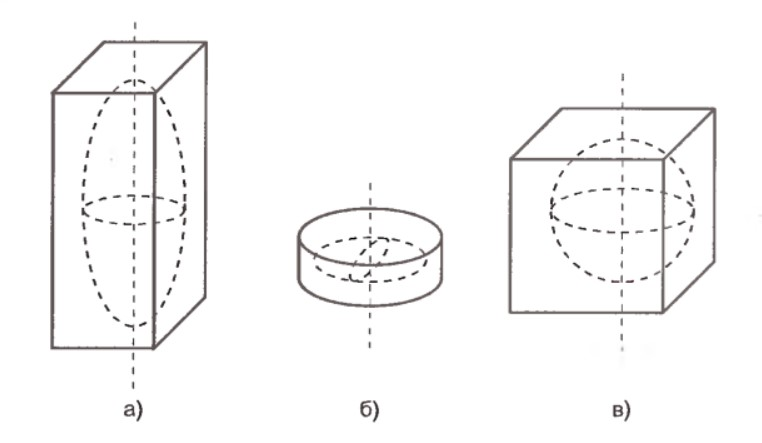
\includegraphics[scale=0.45]{Pics/picture1.jpg} \\
		\textit{\textcolor[HTML]{000000}{Рис. 1. Эллипсоиды инерции параллелепипеда, диска и куба}}
	\end{center}
\end{minipage}  

где $m$ -- суммарная масса системы, $v_c$ -- скорость центра масс системы, а $K$ -- кинетическая энергия точек системы. относительно центра масс. Последнее слагаемое в случае твёрдого тела сводится к вращению тела как целого. Если $v_i$, -- скорость $i$-й точки относительно центра масс, то
\[K = \dfrac{m_i v_i^2}{2}\]
	Cкорость $v_i$, можно представить в виде
\[\vec{v_i} = \vec{\omega} \times \vec{r_i}\]
	Подстановки этого выражения в формулу кинетической энергии точек даёт
\[K = \dfrac{m_i}{2}(\omega \times r_i)^2\]
	Также учтем тождество 
\[(\vec{\omega} \times \vec{r_i})^2 = \omega^2 r_i^2 sin^2 \varphi = \omega^2 r_i^2 (1-cos^2\varphi) = \omega^2 r_i^2 - (\vec{\omega}\cdot\vec{r_i})^2\]
	Поэтому получаем 
\[K = \sum_i \dfrac{m_i}{2}\Big[\omega^2 r_i^2 - (\vec{\omega}\cdot\vec{r_i})^2\Big] =  \dfrac{1}{2}\vec{\omega} \sum_i m_i\Big[\vec{\omega}r_i^2 -(\vec{\omega} \vec{r_i})\vec{r_i} \Big] = \dfrac{1}{2}\vec{\omega}\vec{L},\]
где мы использовалт выражение для момента импульса тела 
\[L=\sum_i m_i\Big[\vec{\omega} r_i^2 - (\vec{\omega}\vec{r_i})\vec{r_i} \Big] = \sum_i m_i\vec{ r} \times (\vec{\omega}\times \vec{r_i}) = \sum_i m_i \vec{r} \times \vec{v_i} \]
	\hspace{0.5cm}Имея в виду связь момента импульса с угловой скоростью, перепишем выражение для кинетической энергии тела в виде
\[K=\dfrac{1}{2}\Big(\vec{\omega},\stackrel{\land}{I}\vec{\omega}\Big)\]
Если $x,y$ и $z$ -- главные оси инерции, то
\begin{equation}
	K =\dfrac{1}{2}\Big(I_x\omega_x^2+I_y\omega_y^2+I_z\omega_z^2\Big)
\end{equation}

В общем случае при вращении тела его главные оси также совершают поворот в пространстве. Это следует учитывать при записи уравнений, определяющих закон изменения компонент вектора угловой скорости со временем.

\vspace{1cm}
{\Large 3. Экспериментальная установка \\}

\noindent\begin{minipage}[c]{0.67\textwidth}
	\hspace{1cm}
	

	В данной работе используется устройство для получения крутильных колебаний,
	изображенных на рисунке 2. Рамка 1 жестко соединена с проволокой 2,
	закрепленной в специальных зажимах 3, позволяющих сообщить начальное закручивание для возбуждения крутильных колебаний вокруг вертикальной оси.
	В рамке с помощью планки 4, гаек 5 и винта 6 закрепляется твердое тело 7. 
	На теле имеются специальные выемки, позволяющие его закрепить так, чтобы ось вращения проходила в теле под различными углами через центр масс.


	Крутильные колебания рамки с телом описываются уравнением:

	\begin{equation}
		(I + I_p)\frac{d^2\phi}{dt^2} = -f\phi.
	\end{equation}
Здесь $I$ и $I_p$ --- моменты инерции тела и рамки относительно оси вращения,
$\phi$ --- угол поворота рамки, меняющийся со временем $t, f$ --- модуль кручения проволоки.
Период крутильных колебаний рамки с телом определяется формулой
\begin{equation}
	T = 2\pi\sqrt{\frac{I + I_p}{f}}.
\end{equation}

\end{minipage}
\begin{minipage}[c]{0.32\textwidth}
	\begin{center}
		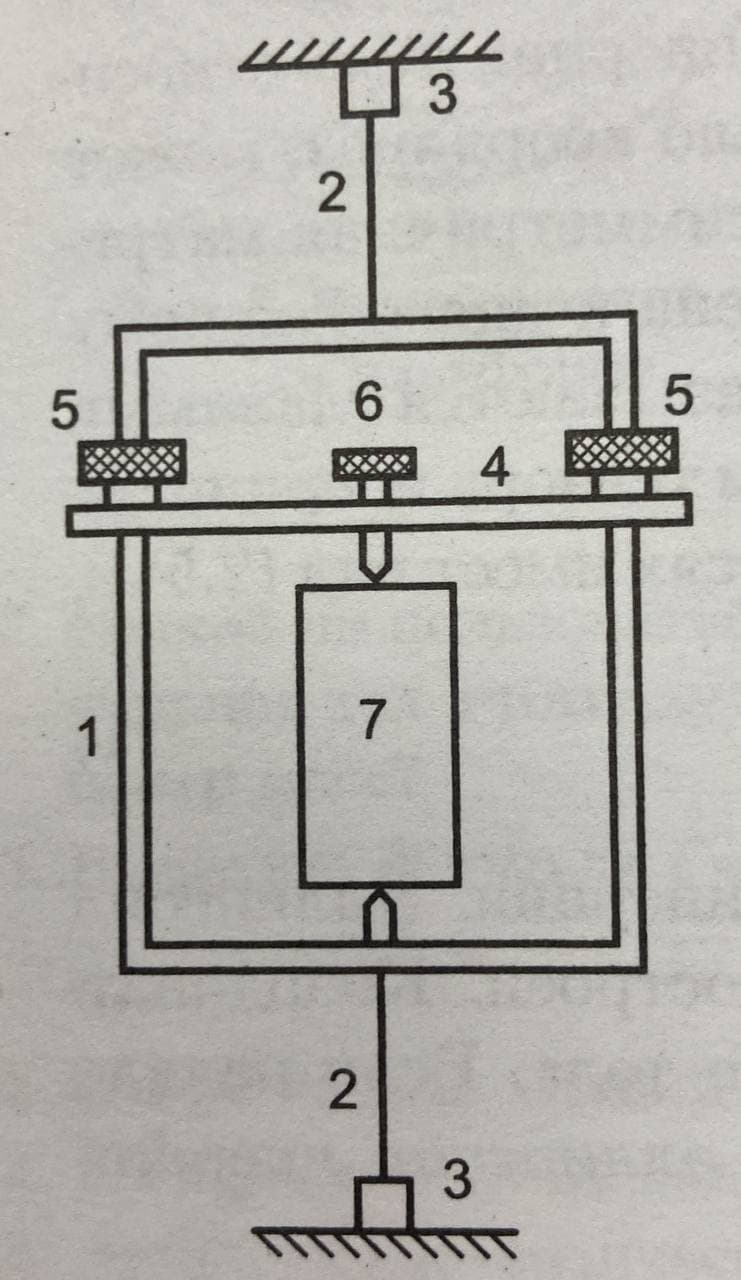
\includegraphics[scale=0.3]{Pics/picture2.jpg} \\
		\textit{\textcolor[HTML]{000000}{Рис. 2. Схема установки}}
	\end{center}
\end{minipage}

\vspace{1cm}
{\Large 4. Инструментальные погрешности \\}
		\textbf{Линейка: } $\sigma_{rul} = \pm 0.5$ мм. (половина цены деления)\\
        \textbf{Электронные весы: } $\sigma_{v} = \pm 0.1$ г (маркировка производителя) \\
        \textbf{Секундомер: } $\sigma_{cnt} = \pm 0.01c$ (цена деления) \\
        \newpage
        Пробный эксперимент:
        \begin{center}
            \begin{tabular}{ | c | c | c | c | c | }
                \hline
                N & Ось & $\tau$, с & n & T, c \\ \hline
                1 & Z & 82.86 & 15 & 5.52 \\ \hline
                2 & Z & 83.68 & 15 & 5.58 \\ \hline
                3 & Z & 83.20 & 15 & 5.55 \\ \hline
                4 & Z & 83.95 & 15 & 5.60 \\ \hline
				5 & Z & 83.18 & 15 & 5.55 \\ \hline
				6 & Z & 83.70 & 15 & 5.58 \\ \hline
            \end{tabular}
            \end{center} 
		Случайную погрешность вычислим по формуле 
		\begin{displaymath}
			\sigma^{ran} = \frac{1}{N}\sqrt{\sum(T - <\overline{T}>)^2}
		\end{displaymath}
        Случайная погрешность равна $\sigma_{ran} = 0.01$.
        Тогда полная погрешность получается равной примерно $\sigma_{full} = 0.02$.
		Соответственно, относительная погрешность будет равна $\epsilon_{full} = 2\%$.

		\vspace{1cm}
        {\Large 5. Результаты измерений и обработка данных }
		Масса параллелепипеда равна: \\
		$m = 2070,6 \pm 0,1$г. \\
		Размеры параллелепипеда равны: \\
		$Z = 150 \pm 0,5$мм. \\
		$Y = 100 \pm 0,5$мм. \\
		$X = 50 \pm 0,5$мм. 

		
		Масса куба равна: \\
		$m = 1083,9 \pm 0,1$г. \\
		Размеры куба равны: \\
		$Z = 93,8 \pm 0,5$мм. \\
		$Y = 93,9 \pm 0,5$мм. \\
		$X = 93,9 \pm 0,5$мм. 
		\begin{center}
            \begin{tabular}{ | c | c | c | c | c | c | }
                \hline
                N & Ось & $\tau$, с & n & T, c & $\frac{1}{\sqrt{T^2-T_0^2}}$ \\ \hline
                1 & Z & 82.86 & 15 & 5.52 & 0.31 \\ \hline
                2 & Z & 83.68 & 15 & 5.58 & 0.30 \\ \hline
                3 & Y & 98.23 & 15 & 6.55 & 0.21 \\ \hline
                4 & Y & 97.82 & 15 & 6.52 & 0.21 \\ \hline
				5 & X & 104.07 & 15 & 6.94 & 0.19 \\ \hline
				6 & X & 105.10 & 15 & 7.00 & 0.19 \\ \hline
				7 & AA' & 89.40 & 15 & 5.96 & 0.25 \\ \hline
				8 & BB' & 90.29 & 15 & 6.02 & 0.25 \\ \hline
				9 & CC' & 89.82 & 15 & 5.98 & 0.25 \\ \hline
				10 & DD' & 89.79 & 15 & 5.98 & 0.25 \\ \hline
				11 & EE' & 86.83 & 15 & 5.79 & 0.27 \\ \hline
				12 & FF' & 86.78 & 15 & 5.79 & 0.27 \\ \hline
				13 & PP' & 88.65 & 15 & 5.91 & 0.26 \\ \hline
				14 & QQ' & 88.77 & 15 & 5.92 & 0.26 \\ \hline
				15 & KK' & 99.05 & 15 & 6.60 & 0.21 \\ \hline
				16 & MM' & 98.81 & 15 & 6.59 & 0.21 \\ \hline
            \end{tabular}
			\captionof{table}{Результаты расчета T для параллелепипеда.}
            \end{center} 
		

			Аналогичная таблица была сделана для куба:

					
		\begin{center}
            \begin{tabular}{ | c | c | c | c | c | c | }
                \hline
                N & Ось & $\tau$, с & n & T, c & $\frac{1}{\sqrt{T^2-T_0^2}}$ \\ \hline
                1 & Z & 79.31 & 15 & 5.29 & 0.35 \\ \hline
                2 & Y & 79.77 & 15 & 5.32 & 0.35 \\ \hline
				3 & X & 79.62 & 15 & 5.31 & 0.36 \\\hline
				4 & AA' & 79.73 & 15 & 5.32 & 0.35 \\ \hline
				5 & BB' & 79.92 & 15 & 5.33 & 0.35 \\ \hline
				6 & CC' & 79.61 & 15 & 5.31 & 0.35 \\ \hline
				7 & DD' & 79.91 & 15 & 5.33 & 0.35 \\\hline
				8 & EE' & 79.58 & 15 & 5.31 & 0.35 \\\hline
				9 & FF' & 80.12 & 15 & 5.34 & 0.34 \\\hline
				10 & PP' & 79.42 & 15 & 5.29 & 0.35 \\\hline
				11 & QQ' & 79.69 & 15 & 5.31 & 0.35 \\\hline
				12 & KK' & 79.58 & 15 & 5.31 & 0.35 \\\hline
				13 & MM' & 79.66 & 15 & 5.31 & 0.35 \\\hline
            \end{tabular}
			\captionof{table}{Результаты расчета T для куба.}
            \end{center}


			Далее на основе полученных данных проверяем формулы: \\
			$1) (a^2 + b^2 + c^2)T_d^2 = a^2T_x^2 + b^2T_y^2 + c^2T_z^2$ \\
			$2) (b^2 + c^2)T_P^2 = b^2T_y^2 + c^2T_z^2$ \\
			$3) (a^2 + c^2)T_F^2 = a^2T_x^2 + c^2T_z^2$ \\
			$4) (a^2 + b^2)T_M^2 = a^2T_x^2 + b^2T_y^2$ \\


			Для параллелепипеда: \\
			$1) 1.254 m^2*c^2 = 1.252 m^2*c^2$ \\
			$2) 1.135 m^2*c^2 = 1.129 m^2*c^2$ \\
			$3) 0.836 m^2*c^2 = 0.823 m^2*c^2$ \\
			$4) 0.542 m^2*c^2 = 0.546 m^2*c^2$ \\
			Для куба: \\
			$1) 0.747 m^2*c^2 = 0.744 m^2*c^2$ \\
			$2) 0.494 m^2*c^2 = 0.496 m^2*c^2$ \\
			$3) 0.496 m^2*c^2 = 0.495 m^2*c^2$ \\
			$4) 0.497 m^2*c^2 = 0.498 m^2*c^2$ \\


			По полученным результатам видно, что все равенства верны в пределах погрешности. 
			Значит, полученные соотношение верны.


			\textbf{Построение эллипсов:} \\
			Чтобы построить сечения эллипсоида, необходимо воспользоваться формулой
			\begin{displaymath}
				G = \frac{1}{\sqrt{T^2 - T_0^2}}
			\end{displaymath}
			где $T_0$ - период крутильный колебаний пустой рамки. $T_0 = 87.2c$.

			\vspace{1cm}
			{\Large 6. Вывод:}


			В ходе данной лабораторной работы над удалось проверить соотношения
			периодов крутильных колебаний двух твердых тел и убедиться в их верности.
			В случае куба мы лишний раз убедились, что все его периоды, а вследствие чего
			и моменты инерции, равны.

			
\end{document}